\pdfminorversion=4
\documentclass[aspectratio=169]{beamer}
\usepackage{animate} % for animation
\usepackage{array,multirow,graphicx}
\usepackage{multicol}
\usepackage{etoolbox}
\graphicspath{{gambar/}}
\setbeamertemplate{caption}[numbered]
\setbeamertemplate{section in toc}[sections numbered]

% Hide subsubsections from TOC, but keep PDF bookmarks with beamer
\hypersetup{bookmarksopen=true,bookmarksopenlevel=4}
\setcounter{tocdepth}{4}

\renewcommand{\figurename}{Gambar.}
\renewcommand{\tablename}{Tabel.}

\usetheme[pageofpages=of,	% String used between the current page and the
							% total page count.
			alternativetitlepage=true,% Use the fancy title page.
			titleline=true,
			titlepagelogo=OK-LOGO-ITK.jpg
%          	 titlepagelogo=fig/jaist_logo.png
			]{Torino}
			% change /beamerinnerthemefancy.sty to resize the logo
\usecolortheme{freewilly}

\makeatletter
\patchcmd{\beamer@sectionintoc}{\vskip1.5em}{\vskip0em}{}{}
\makeatother

\author{Mifta Nur Farid \\
	miftanurfarid@lecturer.itk.ac.id}
\title{RANGKAIAN ELEKTRONIKA II}
\subtitle{Penguat Diferensial}
\institute{Teknik Elektro \\ Institut Teknologi Kalimantan \\ Balikpapan, Indonesia}
\date{\tiny November 24, 2020}

% The log drawn in the upper right corner.
\logo{
\includegraphics[height=0.13\paperheight]{OK-LOGO-ITK.jpg}}

\begin{document}

\begin{frame}[t,plain]
\titlepage
\end{frame}

%\begin{frame}{Bahan Kajian}
%	\begin{multicols}{2} % Two columns for outline
%    \tableofcontents[subsectionstyle=hide]
%	\end{multicols}
%\end{frame}

\section{Pengantar}
\begin{frame}{Pengantar}
	\begin{itemize}
		\item Istilah \textit{Operational amplifier} (op-amp) merujuk kepada sebuah amplifier yang menjalankan suatu operasi matematika.
		\item Dalam sejarahnya, op-amp pertama digunakan di dalam komputer analog untuk melakukan operasi penjumlahan, perkalian dan seterusnya.
		\item Op-amp dibuat sebagai sirkuit diskrit $ \rightarrow $ sekarang kebanyakan op-amp adalah sirkuit terintegrasi/ \textit{integrated circuits} (IC). 
	\end{itemize}
\end{frame}
	
\begin{frame}{Pengantar}
	\begin{itemize}
		\item Op-amp $ \rightarrow $ penguat DC/\textit{DC amplifier} dengan \textit{voltage gain} yang sangat besar, impendansi \textit{input} yang sangat besar, dan impedansi \textit{output} yang sangat kecil.
		\item Frekuensi \textit{Unity gain} dari 1 hingga lebih dari 20 Mhz.
		\item IC op-amp adalah sebuah blok fungsional yang lengkap dengan pin eksternal.
		\item Hanya dengan menghubungkan pin tersebut ke suplai tegangan dan beberapa komponen, kita dapat dengan cepat membuat segala jenis rangkaian yang berguna.
	\end{itemize}
\end{frame}

\begin{frame}{Pengantar}
	\begin{figure}
		\centering
		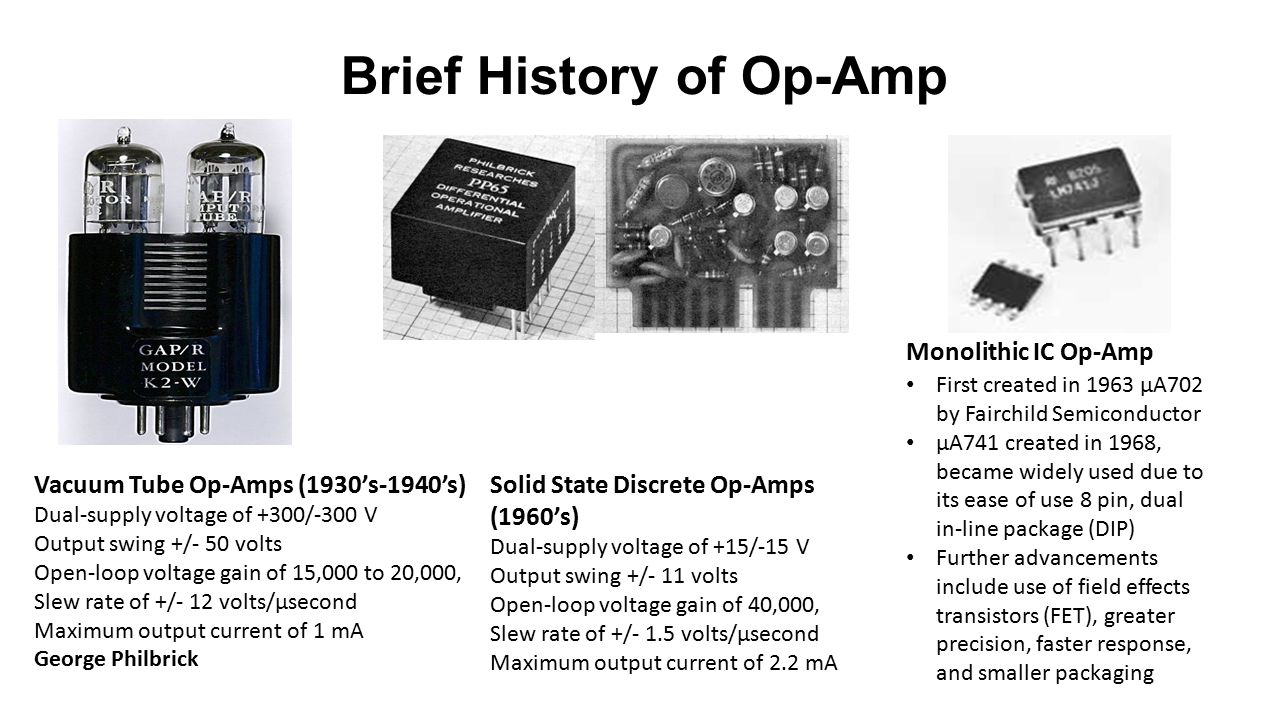
\includegraphics[height=0.75\textheight]{gambar/history-op-amp}
		\caption{Perkembangan op-amp}
		\label{fig:history-op-amp}
	\end{figure}
\end{frame}

\begin{frame}{Pengantar}
	\begin{itemize}
		\item Rangkaian \textit{input} yang paling banyak digunakan di op-amp adalah sebuah penguat diferensial/ \textit{differential amplifier}.
		\item Konfigurasi dari penguat ini memberikan banyak karakteristik \textit{input} di IC.
		\item Penguat diferensial juga dapat dikonfigurasi dalam bentuk diskrit untuk digunakan dalam komunikasi, instrumentasi, dan rangkaian kontrol industri.
		\item \textbf{Kita akan fokus pada penguat diferensial yang digunakan dalam IC.}
	\end{itemize}
\end{frame}

\begin{frame}{Pengantar}
	\begin{itemize}
		\item Sub-CPMK:
		\begin{itemize}
			\item Mahasiswa mampu
menganalisis rangkaian penguat
diferensial (C4, P3, A3)
		\end{itemize}
		\item Bahan Kajian
		\begin{enumerate}
			\item Konsep dasar penguat diferensial;
			\item Analisis DC dari
penguat diferensial;
			\item Analisis AC dari
penguat diferensial;
			\item Common‐mode gain;
		\end{enumerate}
	\end{itemize}
\end{frame}

\begin{frame}{Penguat Diferensial}
	\begin{enumerate}
		\item Transistor, dioda, dan resistor adalah komponen-komponen praktis yang ada di dalam IC.
		\item Kapasitor mungkin dapat digunakan, tapi ukurannya sangat kecil, < 50 pF.
		\item Karena alasan ini, desainer IC tidak bisa menggunakan kapasitor kopling dan bypass.
	\end{enumerate}
\end{frame}
\end{document}

